% =====================================================================
%  Guía de laboratorio — IEL04 — Circuitos Eléctricos I, semana 12
%  Escrita por src/guia_laboratorio.py con la plantilla institucional
%  (config/framework_iub/guia-laboratorio/: guialabiub.sty e img/, copiados a esta carpeta).
%
%  Compilar con:  pdflatex -> biber -> pdflatex -> pdflatex
%  (En Overleaf: compilador pdfLaTeX; biber se ejecuta solo.)
% =====================================================================
\documentclass[12pt]{article}

% Opciones: [sinmarca] quita la marca de agua; [borrador] muestra márgenes
%           [ieee] referencias IEEE (por defecto); [apa] referencias APA 7
\usepackage{guialabiub}

% ------- Tablas, diagramas de flujo, circuitos y gráficas (todo en LaTeX) -------
% (la plantilla no los trae; los estilos y la paleta son los del .tex del temario)
\usepackage{colortbl}                    % encabezado #121023 y filas alternas en las tablas
\usepackage{xltabular}                   % la tabla de materiales se parte entre páginas
\usepackage{tikz}
\usetikzlibrary{arrows.meta,positioning,shapes.geometric,shapes.misc}
\usepackage[siunitx,RPvoltages]{circuitikz}
\usepackage{pgfplots}
\pgfplotsset{compat=1.18}
\usepackage{adjustbox}

% Paleta del Manual de Identidad Visual IUB 2025 (los colores del manual y sus tintes)
\definecolor{iubnavy}{HTML}{121023}
\definecolor{iubyellow}{HTML}{FFDF2D}
\definecolor{iubwhite}{HTML}{FFFFFF}
\definecolor{iubblue}{HTML}{00ADE7}
\definecolor{iuborange}{HTML}{E39037}
\definecolor{iubgreen}{HTML}{3B9C6D}
\colorlet{iubgris}{iubnavy!18}
\colorlet{iubgrisoscuro}{iubnavy!60}
\colorlet{iubfondoazul}{iubblue!8}
\colorlet{iubfondonaranja}{iuborange!10}
\colorlet{iubfondoverde}{iubgreen!9}
\colorlet{iubfondogris}{iubnavy!5}
\colorlet{iubpurple}{iubnavy!45}
\pgfplotsset{cycle list={{iubblue, mark=*},{iuborange, mark=square*},{iubgreen, mark=triangle*},{iubnavy, mark=diamond*},{iubyellow, mark=pentagon*}}}

% Estilos de los diagramas de flujo (TikZ) y de las gráficas (pgfplots)
\tikzset{
  dcaja/.style={draw=iubblue, fill=iubfondoazul, line width=1pt, rounded corners=1pt, align=center, inner sep=2pt, text=iubnavy},
  destado/.style={draw=iubblue, fill=iubfondoazul, line width=1pt, rounded corners=6pt, align=center, inner sep=2pt, text=iubnavy},
  ddecision/.style={draw=iuborange, fill=iubfondonaranja, line width=1pt, diamond, aspect=1.6, align=center, inner sep=1pt, text=iubnavy},
  dterminal/.style={draw=iubgreen, fill=iubfondoverde, line width=1pt, rounded rectangle, align=center, inner sep=2pt, text=iubnavy},
  dflecha/.style={-{Stealth[length=2.4mm]}, line width=0.9pt, draw=iubnavy},
  drotulo/.style={font=\footnotesize, text=iubgrisoscuro, fill=white, fill opacity=0.92, text opacity=1, inner sep=1.5pt},
}
\pgfplotsset{iubejes/.style={width=0.9\linewidth, height=6.2cm, grid=major, grid style={iubgris}, axis lines*=left, axis line style={iubnavy}, tick label style={font=\small}, label style={font=\small}, title style={font=\bfseries\small}, legend cell align=left, legend style={draw=none, fill=none, font=\small, anchor=north, legend columns=-1, /tikz/every even column/.append style={column sep=8pt}}, unbounded coords=jump}}

% --------------------------- Bibliografía ----------------------------
\addbibresource{IEL04-semana12.bib}

% --------------------------- Datos de la guía -------------------------
\facultad{Facultad de Ingenierías}
\modulo{IEL04 --- Circuitos Eléctricos I}
\docente{Ing. Sergio Martinez Castilla}

\begin{document}

% Orden de la bibliografía: el mismo del .md (biblatex numera por orden de primera cita)
\nocite{ref1,ref2,ref3}

\datosguia
\lineablanco

% Título de la práctica y ficha de la sesión
{\centering\bfseries Guía de laboratorio: Circuito RLC en paralelo: corrientes de rama, corriente mínima en la resonancia y circuito tanque con bobina real\par}
\lineablanco
\textbf{Semana:} 12 de 14 \quad \textbf{Resultado de aprendizaje:} IEL04-RA4 \quad \textbf{Práctica:} propuesta a partir de la bibliografía \cite{ref1}, \cite{ref2}, \cite{ref3} \quad \textbf{Duración:} \SI{240}{\minute}
\lineablanco
La práctica corresponde a la sesión teórica de la semana 12, \guillemotleft{}El circuito RLC en paralelo: susceptancias opuestas, ley de corrientes de Kirchhoff, circuito tanque y corrección del factor de potencia\guillemotright{}, y reproduce su caso de estudio: con un resistor de 4,7 k\ensuremath{\Omega}, la bobina L3 y el condensador C2 en paralelo, alimentados con 2,00 V eficaces, se miden las corrientes de rama y la corriente total a 3 kHz, en la resonancia y a 8 kHz, y se observa que en la resonancia la fuente entrega una corriente mínima mientras por la bobina y el condensador circula una corriente mucho mayor. No hay un manual de laboratorio asignado al RA IEL04-RA4, por lo que la práctica se propone a partir de la bibliografía cargada: Floyd trata el análisis y la resonancia en paralelo, incluido el tanque con bobina no ideal \cite{ref1}, Boylestad el circuito resonante en paralelo con la resistencia de la bobina \cite{ref2} y Deorsola la ley de corrientes de Kirchhoff con fasores \cite{ref3}.

% ---------------------------------------------------------------------
\section{Objetivos}\label{sec:objetivos}
\textbf{Objetivo general:} Verificar experimentalmente la ley de corrientes de Kirchhoff y la resonancia en un circuito RLC en paralelo con bobina real.
\lineablanco
\textbf{Objetivos específicos:}
\begin{itemize}
  \item Identificar por su código de colores el resistor y verificar con instrumentos el resistor, la bobina y el condensador. \emph{(CE1)}
  \item Medir las corrientes de las ramas resistiva, inductiva y capacitiva a tres frecuencias. \emph{(CE2)}
  \item Medir la corriente total del circuito RLC en paralelo, localizar su mínimo en la resonancia y compararlo con el cálculo con la bobina real. \emph{(CE3)}
\end{itemize}

% ---------------------------------------------------------------------
\section{Materiales y Equipos}\label{sec:materiales}
% --- Tabla: materiales y equipos (11; xltabular repite el encabezado si se parte) ---
\arrayrulecolor{iubnavy}
\begin{xltabular}{\linewidth}{>{\raggedleft\arraybackslash}p{0.6cm} >{\raggedright\arraybackslash}X >{\raggedright\arraybackslash}X >{\raggedleft\arraybackslash}p{2.2cm}}
\caption{Materiales y equipos de la práctica}\label{tab:materiales} \\
\rowcolor{iubnavy} \textcolor{white}{\textbf{\#}} & \textcolor{white}{\textbf{Material o equipo}} & \textcolor{white}{\textbf{Especificación}} & \textcolor{white}{\textbf{Cantidad}} \\
\endfirsthead
\rowcolor{iubnavy} \textcolor{white}{\textbf{\#}} & \textcolor{white}{\textbf{Material o equipo}} & \textcolor{white}{\textbf{Especificación}} & \textcolor{white}{\textbf{Cantidad}} \\
\endhead
\bottomrule
\endlastfoot
  1 & Resistor & 4,7 k\ensuremath{\Omega} \textpm{}5 \% (amarillo-violeta-rojo-oro) & 1 \\
  \rowcolor{iubfondogris} 2 & Bobina L3 del kit & 103K, 10,4 mH y 24,6 \ensuremath{\Omega} medidos & 1 \\
  3 & Condensador C2 del kit & 104K, 97,8 nF medidos & 1 \\
  \rowcolor{iubfondogris} 4 & Resistor sensor de corriente & 10 \ensuremath{\Omega} & 1 \\
  5 & Generador de funciones & --- & 1 \\
  \rowcolor{iubfondogris} 6 & Osciloscopio de dos canales con puntas \texttimes{}10 & --- & 1 \\
  7 & Multímetro digital de verdadero valor eficaz & --- & 2 \\
  \rowcolor{iubfondogris} 8 & Medidor LCR & --- & 1 \\
  9 & Protoboard & --- & 1 \\
  \rowcolor{iubfondogris} 10 & Cables de conexión & --- & 12 \\
  11 & Resistencia de descarga & 1 k\ensuremath{\Omega} & 1 \\
\end{xltabular}

% ---------------------------------------------------------------------
\section{Procedimiento}\label{sec:procedimiento}
La práctica ocupa el bloque de 2 h de laboratorio de la sesión y se realiza en grupos de tres estudiantes, con tres roles que rotan entre etapas: quien monta y opera el circuito, quien mide y quien registra y verifica los cálculos. Antes de energizar cualquier montaje, el docente o el monitor revisa la conexión. Cada etapa abre con su diagrama de flujo, que muestra la secuencia y las comprobaciones de un vistazo, y sigue con sus pasos numerados; cada paso indica cuánto dura, qué debe observarse para saber que salió bien y qué hacer si no. Los valores numéricos de la sesión teórica sirven de referencia: las lecturas propias del grupo se registran en las tablas de la sección de análisis.
\lineablanco
% --- Etapa 1: Preparación y predicción (5 pasos) ---
\subsection{Preparación y predicción (\SI{35}{\minute})}\label{sec:etapa-1}
% --- Figura 1: diagrama de flujo de la etapa 1 (TikZ, con la paleta IUB) ---
\begin{figure}[H]
  \centering
\begin{adjustbox}{max width=\linewidth}
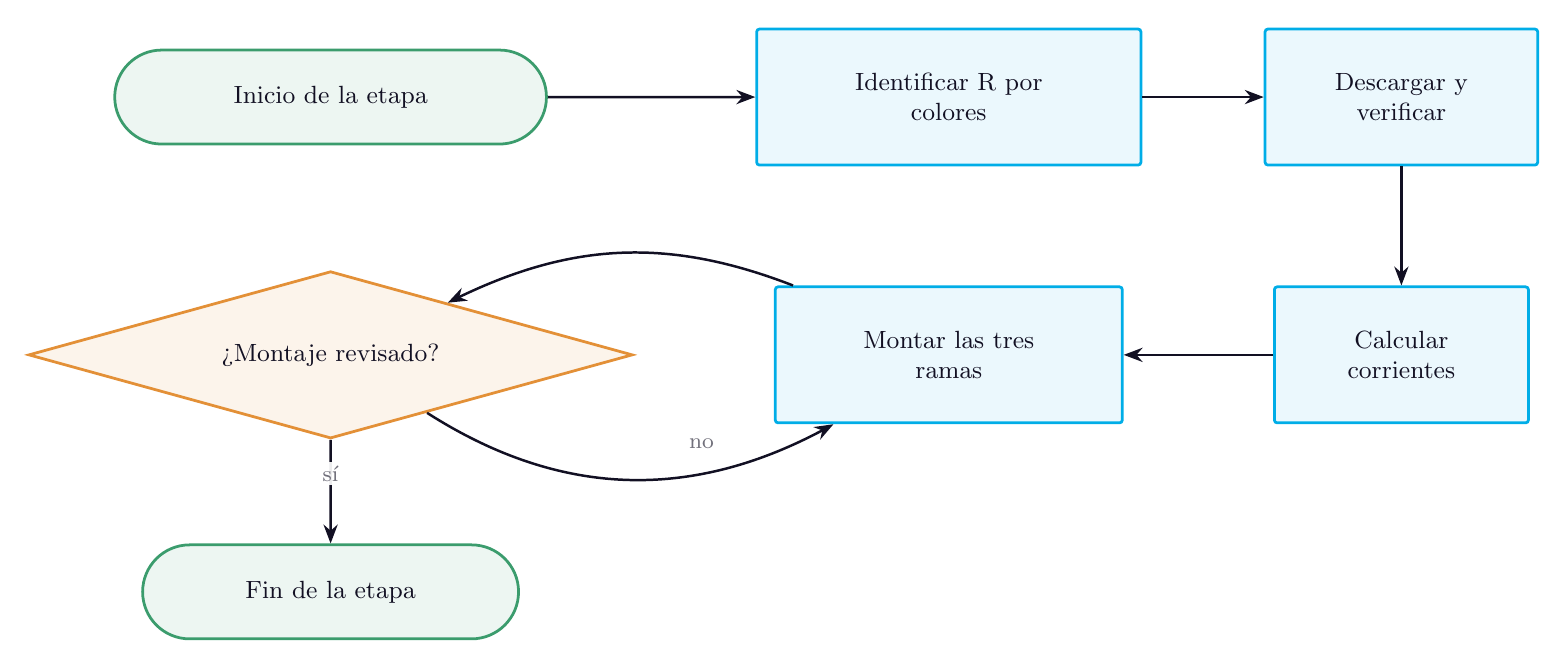
\begin{tikzpicture}[x=1in, y=1in, font=\small]
  % nodos (centro en pulgadas, con el tamano que calcula figuras.py)
  \node[dterminal, minimum width=2.214in, minimum height=0.470in] (n0) at (1.510,-0.340) {Inicio de la etapa};  % ini
  \node[dcaja, minimum width=1.921in, minimum height=0.680in] (n1) at (4.601,-0.340) {Identificar R por \\ colores};  % a0
  \node[dcaja, minimum width=1.363in, minimum height=0.680in] (n2) at (6.864,-0.340) {Descargar y \\ verificar};  % a1
  \node[dcaja, minimum width=1.270in, minimum height=0.680in] (n3) at (6.864,-1.629) {Calcular \\ corrientes};  % a2
  \node[dcaja, minimum width=1.735in, minimum height=0.680in] (n4) at (4.601,-1.629) {Montar las tres \\ ramas};  % a3
  \node[ddecision, minimum width=3.021in, minimum height=0.799in] (n5) at (1.510,-1.629) {\textquestiondown{}Montaje revisado?};  % dec
  \node[dterminal, minimum width=1.935in, minimum height=0.470in] (n6) at (1.510,-2.814) {Fin de la etapa};  % fin
  % flechas (las de retorno, curvas)
  \draw[dflecha] (n0) -- (n1);
  \draw[dflecha] (n1) -- (n2);
  \draw[dflecha] (n2) -- (n3);
  \draw[dflecha] (n3) -- (n4);
  \draw[dflecha] (n4) to[bend right=24] (n5);
  \draw[dflecha] (n5) -- (n6);
  \draw[dflecha] (n5) to[bend right=31] (n4);
  % rotulos de las flechas (donde no caen sobre un nodo)
  \node[drotulo] at (1.510,-2.222) {sí};
  \node[drotulo] at (3.365,-2.075) {no};
\end{tikzpicture}
\end{adjustbox}
  \caption{Diagrama de flujo de la etapa 1: Preparación y predicción}
  \label{fig:flujo-1}
\end{figure}
\begin{pasos}
  \item \textbf{Paso~1:} Identificar el resistor por su código de colores (amarillo-violeta-rojo-oro: 4,7 k\ensuremath{\Omega} \textpm{}5 \%) \cite{ref1}. \emph{(aprox.~\SI{3}{\minute})} \textbf{Comprobación:} Si no da 4,7 k\ensuremath{\Omega}, revisar el sentido de lectura.
  \item \textbf{Paso~2:} Descargar el condensador conectando entre sus terminales, durante unos segundos, una resistencia de 1 k\ensuremath{\Omega} sujeta con pinzas aisladas, y medir con el voltímetro en cd la tensión entre terminales. \emph{(aprox.~\SI{3}{\minute})} \textbf{Comprobación:} La tensión debe ser prácticamente nula (menos de 0,1 V); si no lo es, repetir la descarga antes de manipular el componente. \textbf{Seguridad:} No cortocircuitar los terminales con los dedos ni con una herramienta metálica: un condensador puede conservar carga después de desconectado.
  \item \textbf{Paso~3:} Verificar el resistor con el ohmímetro, la bobina L3 con el medidor LCR y el ohmímetro (10,4 mH y 24,6 \ensuremath{\Omega} esperados) y el condensador C2 con el medidor LCR (97,8 nF esperados). \emph{(aprox.~\SI{8}{\minute})} \textbf{Comprobación:} Si algún valor difiere más que su tolerancia del registrado, anotar el nuevo valor y rehacer el cálculo previo con él.
  \item \textbf{Paso~4:} Calcular con los valores medidos la corriente de cada rama y la corriente total a 3 kHz, en la resonancia y a 8 kHz, sumando las admitancias en forma rectangular con la bobina real. \emph{(aprox.~\SI{15}{\minute})} \textbf{Comprobación:} En la resonancia la corriente total esperada es cercana a 0,89 mA, muy inferior a la de la bobina o el condensador (unos 6,1 mA).
% ecuación del paso 4: Resistencia equivalente en paralelo de la bobina real:
\par Resistencia equivalente en paralelo de la bobina real:
\begin{equation}
  R_{p(eq)} = R_W \left(Q^2 + 1\right)
  \label{eq:paso-4}
\end{equation}
donde $R_{p(eq)}$ y $R_W$ en ohmios (\ensuremath{\Omega}); $Q = X_L / R_W$ adimensional.
  \item \textbf{Paso~5:} Montar las tres ramas en paralelo y el resistor sensor en serie con la fuente del lado de tierra. \emph{(aprox.~\SI{6}{\minute})} \textbf{Comprobación:} El docente revisa el montaje antes de energizar. \textbf{Seguridad:} Montar con el generador apagado.
% figura del paso 5: Circuito RLC en paralelo con el amperímetro en serie con la fuente (circuito en circuitikz)
\par\medskip\noindent
\begin{minipage}{\linewidth}
  \centering
  \begin{adjustbox}{max width=\linewidth}
    \begin{circuitikz}[color=iubnavy]
    \draw (0,0) to[sV, l=$v_s$] (0,3) to[ammeter, l=$I_T$] (3,3) to[R, l=$R$] (3,0) -- (0,0); \draw (3,3) -- (5.5,3) to[L, l=$L_3$] (5.5,0) -- (3,0); \draw (5.5,3) -- (8,3) to[C, l=$C_2$] (8,0) -- (5.5,0); \draw (0,0) node[ground]{};
    \end{circuitikz}
  \end{adjustbox}
  \captionof{figure}{Circuito RLC en paralelo con el amperímetro en serie con la fuente}\label{fig:paso-5}
\end{minipage}
\par\medskip
\end{pasos}
% --- Etapa 2: Corrientes a 3 kHz y 8 kHz (3 pasos) ---
\subsection{Corrientes a 3 kHz y 8 kHz (\SI{33}{\minute})}\label{sec:etapa-2}
% --- Figura 3: diagrama de flujo de la etapa 2 (TikZ, con la paleta IUB) ---
\begin{figure}[H]
  \centering
\begin{adjustbox}{max width=\linewidth}
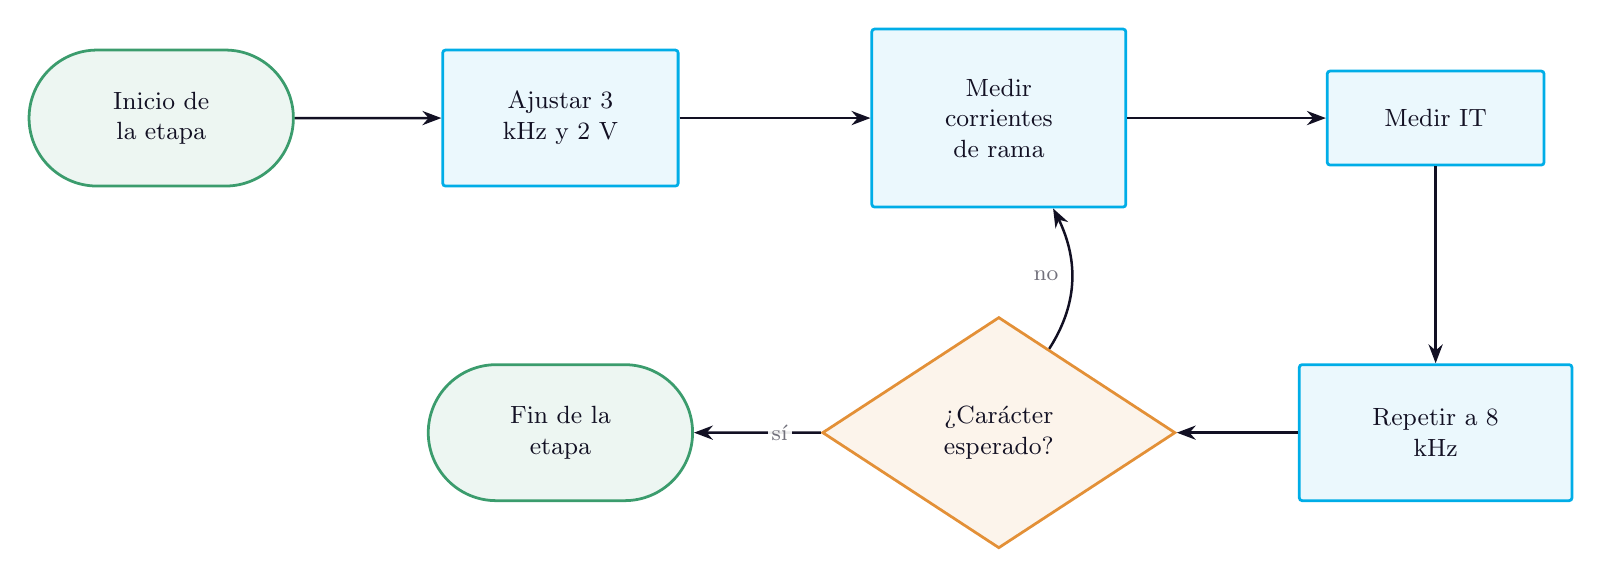
\begin{tikzpicture}[x=1in, y=1in, font=\small]
  % nodos (centro en pulgadas, con el tamano que calcula figuras.py)
  \node[dterminal, minimum width=1.377in, minimum height=0.680in] (n0) at (0.689,-0.445) {Inicio de \\ la etapa};  % ini
  \node[dcaja, minimum width=1.177in, minimum height=0.680in] (n1) at (2.685,-0.445) {Ajustar 3 \\ kHz y 2 V};  % a0
  \node[dcaja, minimum width=1.270in, minimum height=0.890in] (n2) at (4.877,-0.445) {Medir \\ corrientes \\ de rama};  % a1
  \node[dcaja, minimum width=1.084in, minimum height=0.470in] (n3) at (7.061,-0.445) {Medir IT};  % a2
  \node[dcaja, minimum width=1.363in, minimum height=0.680in] (n4) at (7.061,-2.018) {Repetir a 8 \\ kHz};  % a3
  \node[ddecision, minimum width=1.766in, minimum height=1.156in] (n5) at (4.877,-2.018) {\textquestiondown{}Carácter \\ esperado?};  % dec
  \node[dterminal, minimum width=1.377in, minimum height=0.680in] (n6) at (2.685,-2.018) {Fin de la \\ etapa};  % fin
  % flechas (las de retorno, curvas)
  \draw[dflecha] (n0) -- (n1);
  \draw[dflecha] (n1) -- (n2);
  \draw[dflecha] (n2) -- (n3);
  \draw[dflecha] (n3) -- (n4);
  \draw[dflecha] (n4) -- (n5);
  \draw[dflecha] (n5) -- (n6);
  \draw[dflecha] (n5) to[bend right=31] (n2);
  % rotulos de las flechas (donde no caen sobre un nodo)
  \node[drotulo] at (3.781,-2.018) {sí};
  \node[drotulo] at (5.113,-1.232) {no};
\end{tikzpicture}
\end{adjustbox}
  \caption{Diagrama de flujo de la etapa 2: Corrientes a 3 kHz y 8 kHz}
  \label{fig:flujo-2}
\end{figure}
\begin{pasos}
  \item \textbf{Paso~6:} Ajustar el generador a una onda sinusoidal de 3 kHz y medir con el osciloscopio y con el multímetro de verdadero valor eficaz que la tensión en los bornes del circuito, con el circuito conectado, sea de 2,00 V eficaces. \emph{(aprox.~\SI{6}{\minute})} \textbf{Comprobación:} El multímetro debe indicar 2,00 V y el osciloscopio una sinusoide sin distorsión; si la tensión baja al conectar el circuito, reajustar la amplitud con el circuito conectado.
  \item \textbf{Paso~7:} Con el circuito desenergizado, insertar el amperímetro en cada rama y en serie con la fuente, energizando para cada lectura, y anotar $I_R$, $I_{\mathrm{bob}}$, $I_C$ e $I_T$. \emph{(aprox.~\SI{15}{\minute})} \textbf{Comprobación:} A 3 kHz la corriente de la bobina debe superar a la del condensador (carácter inductivo). \textbf{Seguridad:} Insertar el amperímetro solo con el circuito desenergizado.
  \item \textbf{Paso~8:} Repetir las cuatro lecturas a 8 kHz, reajustando la tensión de la fuente. \emph{(aprox.~\SI{12}{\minute})} \textbf{Comprobación:} A 8 kHz la corriente del condensador debe superar a la de la bobina (carácter capacitivo).
\end{pasos}
% --- Etapa 3: Corriente mínima en la resonancia (2 pasos) ---
\subsection{Corriente mínima en la resonancia (\SI{20}{\minute})}\label{sec:etapa-3}
% --- Figura 4: diagrama de flujo de la etapa 3 (TikZ, con la paleta IUB) ---
\begin{figure}[H]
  \centering
\begin{adjustbox}{max width=\linewidth}
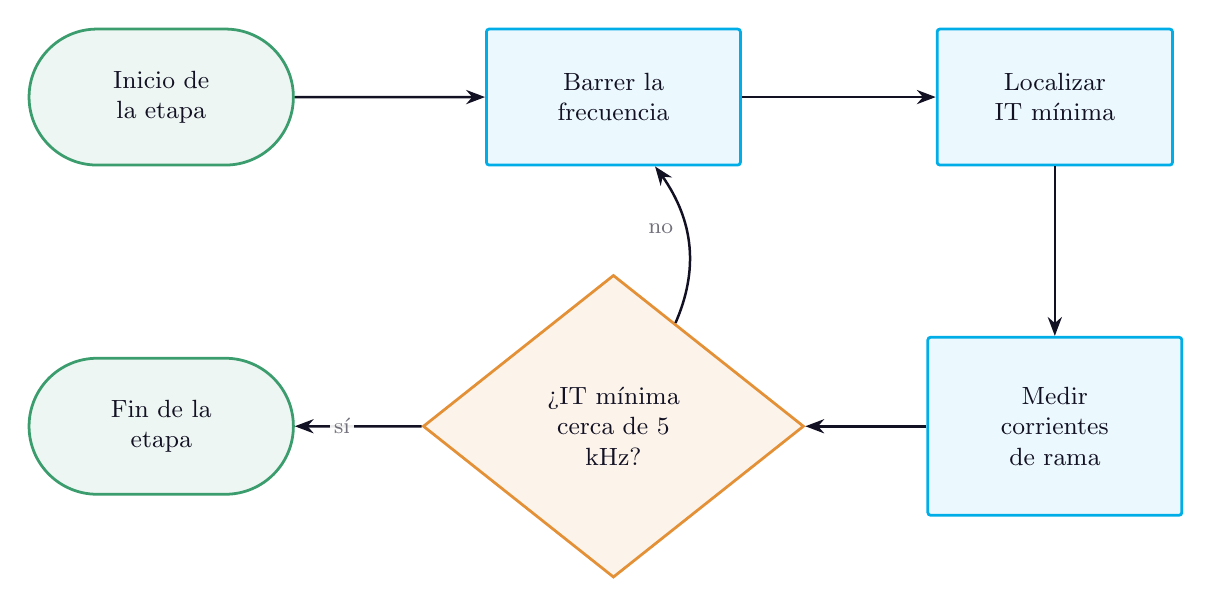
\begin{tikzpicture}[x=1in, y=1in, font=\small]
  % nodos (centro en pulgadas, con el tamano que calcula figuras.py)
  \node[dterminal, minimum width=1.377in, minimum height=0.680in] (n0) at (0.689,-0.340) {Inicio de \\ la etapa};  % ini
  \node[dcaja, minimum width=1.270in, minimum height=0.680in] (n1) at (2.950,-0.340) {Barrer la \\ frecuencia};  % a0
  \node[dcaja, minimum width=1.177in, minimum height=0.680in] (n2) at (5.157,-0.340) {Localizar \\ IT mínima};  % a1
  \node[dcaja, minimum width=1.270in, minimum height=0.890in] (n3) at (5.157,-1.986) {Medir \\ corrientes \\ de rama};  % a2
  \node[ddecision, minimum width=1.905in, minimum height=1.513in] (n4) at (2.950,-1.986) {\textquestiondown{}IT mínima \\ cerca de 5 \\ kHz?};  % dec
  \node[dterminal, minimum width=1.377in, minimum height=0.680in] (n5) at (0.689,-1.986) {Fin de la \\ etapa};  % fin
  % flechas (las de retorno, curvas)
  \draw[dflecha] (n0) -- (n1);
  \draw[dflecha] (n1) -- (n2);
  \draw[dflecha] (n2) -- (n3);
  \draw[dflecha] (n3) -- (n4);
  \draw[dflecha] (n4) -- (n5);
  \draw[dflecha] (n4) to[bend right=31] (n1);
  % rotulos de las flechas (donde no caen sobre un nodo)
  \node[drotulo] at (1.593,-1.986) {sí};
  \node[drotulo] at (3.187,-0.999) {no};
\end{tikzpicture}
\end{adjustbox}
  \caption{Diagrama de flujo de la etapa 3: Corriente mínima en la resonancia}
  \label{fig:flujo-3}
\end{figure}
\begin{pasos}
  \item \textbf{Paso~9:} Con el amperímetro en serie con la fuente, barrer la frecuencia entre 3 kHz y 8 kHz y localizar el mínimo de la corriente total, reajustando la fuente a 2,00 V eficaces. \emph{(aprox.~\SI{10}{\minute})} \textbf{Comprobación:} El mínimo debe aparecer cerca de 5 kHz \cite{ref1}; si la corriente no baja, revisar la rama del condensador.
  \item \textbf{Paso~10:} Anotar la frecuencia del mínimo y medir en ella las corrientes de las tres ramas. \emph{(aprox.~\SI{10}{\minute})} \textbf{Comprobación:} La corriente de la bobina y la del condensador deben ser varias veces la corriente total: es la corriente de circulación del tanque.
\end{pasos}
% --- Etapa 4: Desmontaje y cierre (3 pasos) ---
\subsection{Desmontaje y cierre (\SI{10}{\minute})}\label{sec:etapa-4}
% --- Figura 5: diagrama de flujo de la etapa 4 (TikZ, con la paleta IUB) ---
\begin{figure}[H]
  \centering
\begin{adjustbox}{max width=\linewidth}
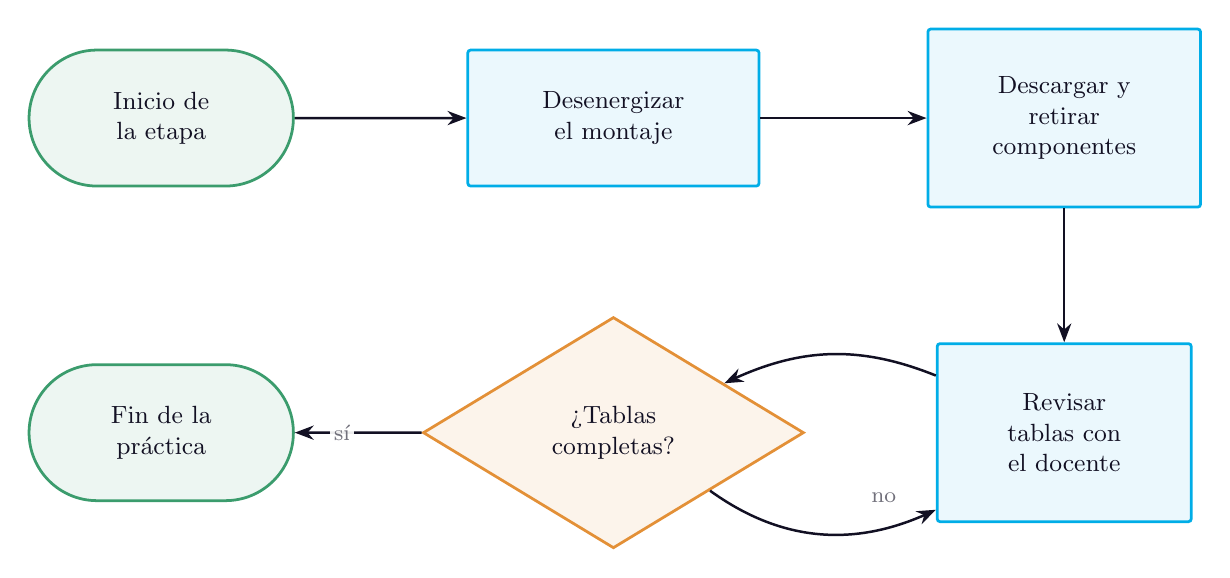
\begin{tikzpicture}[x=1in, y=1in, font=\small]
  % nodos (centro en pulgadas, con el tamano que calcula figuras.py)
  \node[dterminal, minimum width=1.377in, minimum height=0.680in] (n0) at (0.689,-0.445) {Inicio de \\ la etapa};  % ini
  \node[dcaja, minimum width=1.456in, minimum height=0.680in] (n1) at (2.950,-0.445) {Desenergizar \\ el montaje};  % a0
  \node[dcaja, minimum width=1.363in, minimum height=0.890in] (n2) at (5.204,-0.445) {Descargar y \\ retirar \\ componentes};  % a1
  \node[dcaja, minimum width=1.270in, minimum height=0.890in] (n3) at (5.204,-2.018) {Revisar \\ tablas con \\ el docente};  % a2
  \node[ddecision, minimum width=1.905in, minimum height=1.156in] (n4) at (2.950,-2.018) {\textquestiondown{}Tablas \\ completas?};  % dec
  \node[dterminal, minimum width=1.377in, minimum height=0.680in] (n5) at (0.689,-2.018) {Fin de la \\ práctica};  % fin
  % flechas (las de retorno, curvas)
  \draw[dflecha] (n0) -- (n1);
  \draw[dflecha] (n1) -- (n2);
  \draw[dflecha] (n2) -- (n3);
  \draw[dflecha] (n3) to[bend right=24] (n4);
  \draw[dflecha] (n4) -- (n5);
  \draw[dflecha] (n4) to[bend right=31] (n3);
  % rotulos de las flechas (donde no caen sobre un nodo)
  \node[drotulo] at (1.593,-2.018) {sí};
  \node[drotulo] at (4.302,-2.343) {no};
\end{tikzpicture}
\end{adjustbox}
  \caption{Diagrama de flujo de la etapa 4: Desmontaje y cierre}
  \label{fig:flujo-4}
\end{figure}
\begin{pasos}
  \item \textbf{Paso~11:} Apagar el generador de funciones y la fuente, desconectar las puntas del osciloscopio y retirar la alimentación del protoboard. \emph{(aprox.~\SI{3}{\minute})} \textbf{Comprobación:} Ningún indicador de salida debe quedar encendido en el generador ni en la fuente. \textbf{Seguridad:} Desenergizar siempre antes de retirar componentes.
  \item \textbf{Paso~12:} Descargar los condensadores del montaje con la resistencia de descarga, retirar los componentes y devolverlos al kit del grupo con su rótulo. \emph{(aprox.~\SI{4}{\minute})} \textbf{Comprobación:} El kit debe quedar completo, con cada componente en su lugar y con su valor medido anotado.
  \item \textbf{Paso~13:} Revisar con el docente las tablas de registro antes de abandonar el banco. \emph{(aprox.~\SI{3}{\minute})} \textbf{Comprobación:} Las tablas deben estar completas y con unidades; si falta un dato, repetir esa medición antes de desmontar el instrumento.
\end{pasos}

% ---------------------------------------------------------------------
\section{Cuestiones a Resolver}\label{sec:cuestiones}
\begin{enumerate}
  \item \textquestiondown{}Por qué en la resonancia la corriente total es menor que la corriente de la bobina o la del condensador?
  \item \textquestiondown{}Cómo explica la resistencia de devanado que la corriente mínima medida sea mayor que la que predice el modelo ideal?
  \item \textquestiondown{}Cómo se obtiene la resistencia equivalente en paralelo de la bobina real, $R_{p(eq)} = R_W(Q^2 + 1)$, y qué valor da con los datos medidos \cite{ref1}?
  \item \textquestiondown{}Cómo cambia el carácter del circuito al pasar por la resonancia, y cómo se observó en las corrientes?
\end{enumerate}

% ---------------------------------------------------------------------
\section{Análisis de Resultados}\label{sec:analisis}
Presentar en la tabla de registro las corrientes calculadas con la bobina real y las medidas a las tres frecuencias, con su diferencia porcentual y el carácter del circuito en cada una.
\lineablanco
Dibujar el diagrama fasorial de corrientes en la resonancia y a 3 kHz, y comprobar que la suma fasorial de las corrientes de rama reproduce la corriente total medida, mientras su suma aritmética la supera ampliamente.
% --- Tabla de registro 1: RLC en paralelo con VS = 2,00 V eficaces (4 filas vacías para registrar en el banco) ---
\begin{table}[H]
  \centering
  \caption{RLC en paralelo con VS = 2,00 V eficaces}
  \label{tab:registro-1}
  \arrayrulecolor{iubnavy}
  \begin{tabularx}{\linewidth}{>{\raggedright\arraybackslash}X>{\raggedright\arraybackslash}X>{\raggedright\arraybackslash}X>{\raggedright\arraybackslash}X>{\raggedright\arraybackslash}X>{\raggedright\arraybackslash}X}
    \rowcolor{iubnavy} \textcolor{white}{\textbf{Frecuencia (kHz)}} & \textcolor{white}{\textbf{IR (mA)}} & \textcolor{white}{\textbf{Ibob (mA)}} & \textcolor{white}{\textbf{IC (mA)}} & \textcolor{white}{\textbf{IT (mA)}} & \textcolor{white}{\textbf{Carácter}} \\
    \rule{0pt}{0.8cm} & & & & & \\
    \rowcolor{iubfondogris} \rule{0pt}{0.8cm} & & & & & \\
    \rule{0pt}{0.8cm} & & & & & \\
    \rowcolor{iubfondogris} \rule{0pt}{0.8cm} & & & & & \\
    \bottomrule
  \end{tabularx}
\end{table}

% ---------------------------------------------------------------------
\section{Conclusiones}\label{sec:conclusiones}
Concluir si las corrientes medidas cumplen la ley de corrientes de Kirchhoff en forma fasorial y cómo se manifiesta la resonancia en paralelo, explicando el papel de la resistencia de devanado en la corriente mínima; relacionar la práctica con los criterios de medición en circuitos RLC del RA.
\lineablanco
\begin{itemize}
  \item \textquestiondown{}Qué tan cerca estuvo la frecuencia del mínimo de la calculada?
  \item \textquestiondown{}Qué aprendieron sobre la corriente de circulación del tanque?
  \item \textquestiondown{}Por qué el modelo con bobina ideal no basta para predecir la corriente mínima?
\end{itemize}

% ---------------------------------------------------------------------
\section{Recomendaciones de Seguridad}\label{sec:seguridad}
\begin{itemize}
  \item Trabajar con el circuito desenergizado mientras se conecta o modifica el montaje; energizar solo después de la revisión del docente.
  \item Conectar las tierras de las dos puntas del osciloscopio a un mismo nodo de referencia: unirlas a nodos distintos cortocircuita el elemento que queda entre ellas.
  \item Insertar el amperímetro en serie con la rama solo con el circuito desenergizado y con el instrumento en la función y la escala de corriente; nunca conectarlo en paralelo con la fuente.
  \item Reajustar la tensión de la fuente después de cada cambio de frecuencia y no superar los 2,00 V eficaces previstos.
\end{itemize}

% ---------------------------------------------------------------------
\section{Bibliografía}\label{sec:bibliografia}
% Las fuentes cargadas se citan en el texto con \cite{refN}; el \nocite del principio fija su orden y \nocite{*} incluye las demás del .bib.
\nocite{*}
\bibliografia

\end{document}
